\documentclass{beamer}

\usepackage[utf8]{inputenc}
\usepackage{graphicx}
\graphicspath{ {./Figures/} }

\title{Modeling Price and Popularity of AirBnB listings in New-York}
\author{Olivier Binette, Raphael Morsomme}
\institute{Department of Statistical Science, Duke University}
\date{02/20/2020}

\begin{document}

\frame{\titlepage}


\begin{frame} \frametitle{test}    
    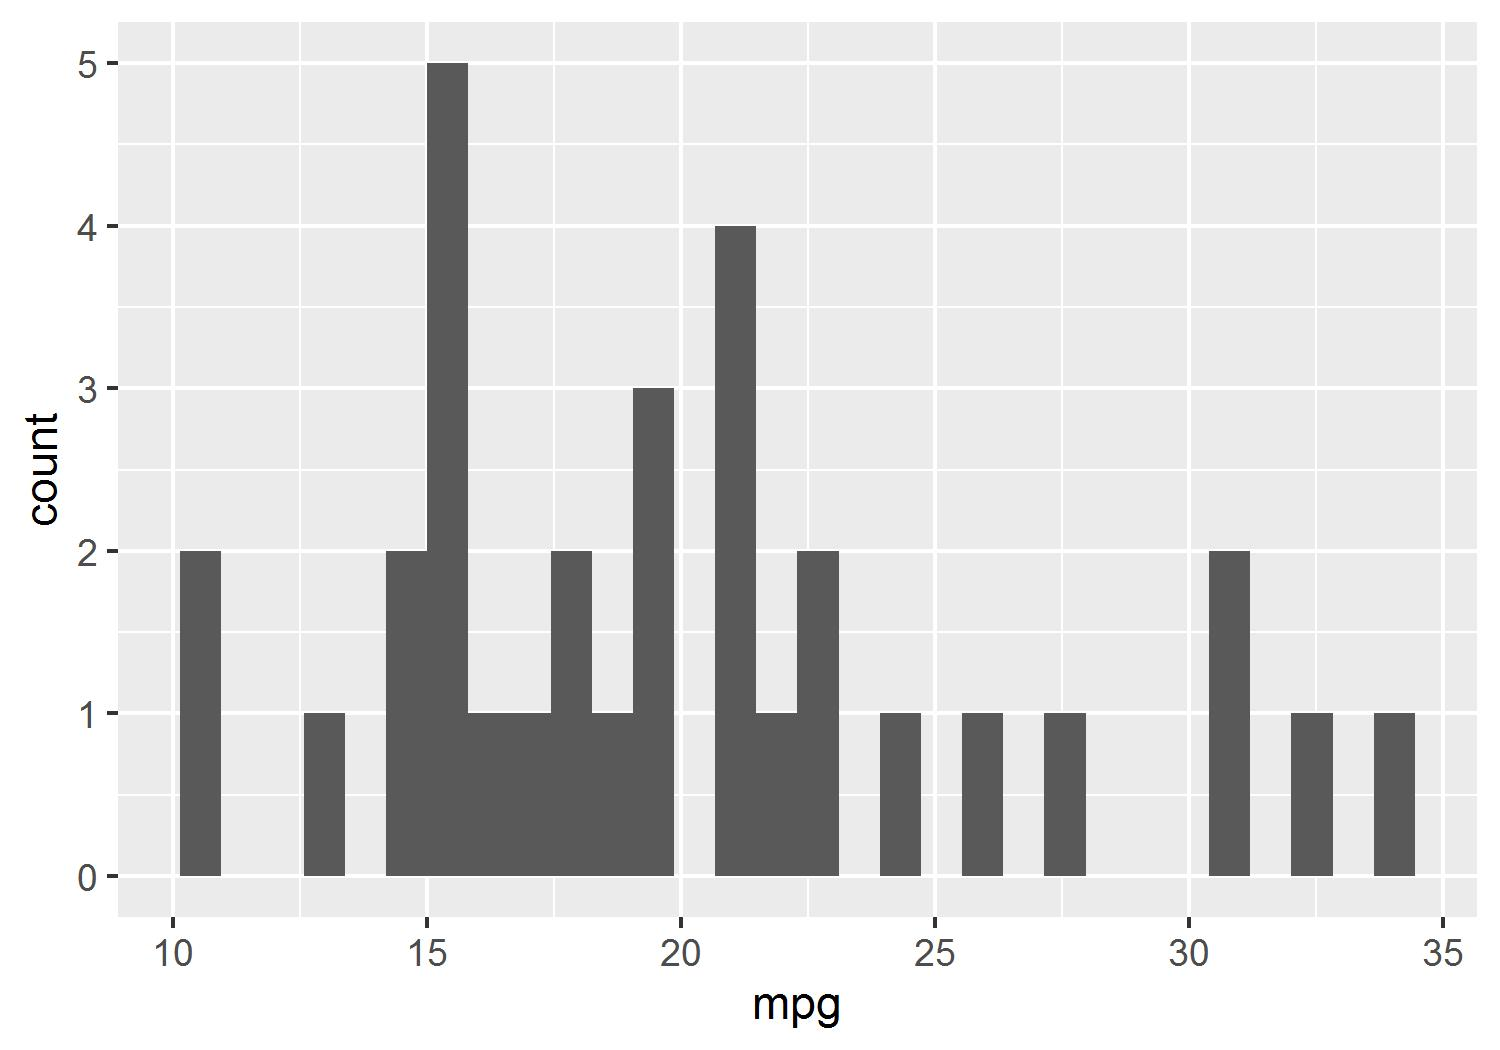
\includegraphics[scale = 0.8]{test.jpeg}
\end{frame}

\begin{frame} \frametitle{Conformal Predictors}

Prediction intervals that are
\begin{itemize}
	\item valid at a given significance level for \textit{finite} sample.
	\item distribution-free
	\item universal
	\item individualized
	\item only assume exchangeability
	\item much more efficient than bootstrap (only fit model once).
\end{itemize}
\end{frame}


\begin{frame} \frametitle{Inductive Conformal Prediction}

Given a labeled training set $\{z_i = (x_i, y_i)\}_{i=1}^n$ and an unlabeled test observation $x_{n+1}$,
\begin{enumerate}
	\item partition training set into a \textit{proper training} set $\{z_i\}_{i=1}^k$ and a \textit{calibration} set $\{z_i \}_{i=k+1}^n$
	\item fit predictive model on proper training set
	\item compute prediction on calibration set and compute anomaly scores
	$$a(z_j) = |\hat{y}_j - y_j|, j = k+1, \dots, n$$
	\item compute prediction on test observation and set the prediction interval to be
	$$\{y: |\hat{y}_{n+1} - y| < a_\epsilon\}$$
	where $a_\epsilon$ is the $\epsilon^{\text{th}}$ percentile of the $\{a\}_{i=k+1}^n$.
	\end{enumerate}
\end{frame}


\begin{frame} \frametitle{Set up}
\begin{itemize}
	\item Use a $10\%$ test set to evaluate the tightness of the prediction intervals and repeat $100$ times.
	\item Calibration set is $30\%$ of training set.
\end{itemize}
\end{frame}





\begin{frame}
\frametitle{References}
\footnotesize{
	\begin{thebibliography}{99} % Beamer does not support BibTeX so references must be inserted manually as below
		
		\bibitem[Whickam, 2013]{Whickam2009} Whickam, H. \\
		\newblock Tidy Data\\
		\newblock \emph{Journal}, month year
		
		\bibitem[Valente, 2005]{Valente2005} Valente, j. \\
		\newblock Apartment Rent Prediction Using Spatial Modeling\\
		\newblock \emph{Journal}, month year
		
		\bibitem[Belasco, 2012]{Belasco2012} Belasco, E. \\
		\newblock Using a Finite Mixture Model of Heterogeneous Households to Delineate Housing Submarkets\\
		\newblock \emph{Journal}, month year
		
	\end{thebibliography}
}
\end{frame}
    






\end{document}
